\documentclass{amsart}

\usepackage{pdflscape}
\usepackage{rotating}

\usepackage{tikz}
\usetikzlibrary{calc,fadings,patterns,decorations.pathmorphing}

\begin{document}

\begin{landscape}
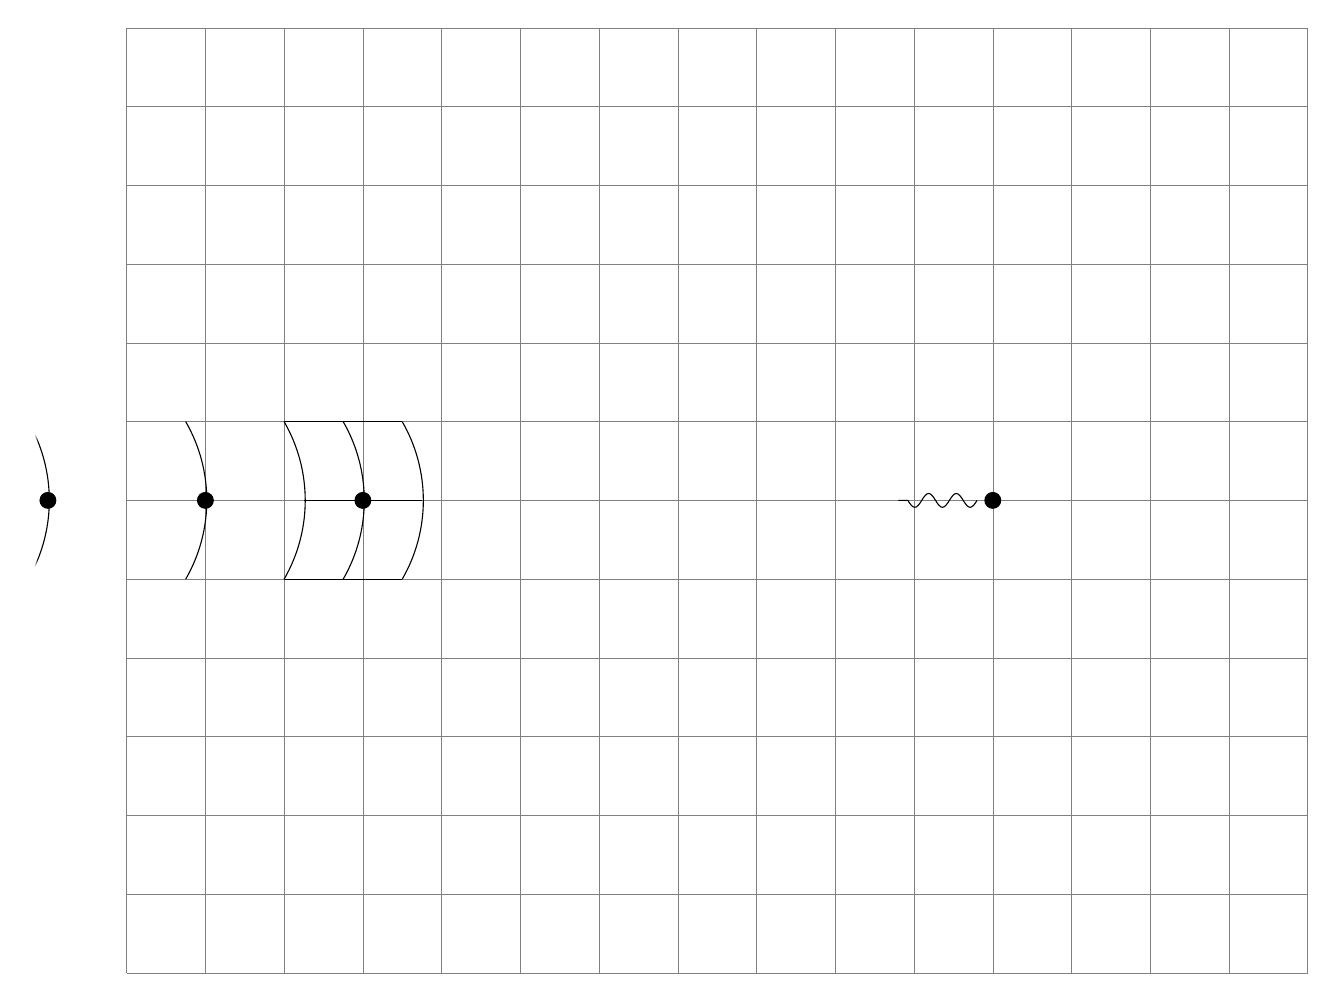
\begin{tikzpicture}
% draw grid
\draw[step=1cm,gray,very thin] (-1,-6) grid (14,6);

% draw Spec Z_(p)
\begin{scope}[shift={(-2cm,0)}]
\draw[fill=black] (0,0) circle (0.1cm);
\draw[path fading=circle with fuzzy edge 20 percent,black] (-0.25,-1) arc (-30:30:2cm);
\end{scope}

% draw M_fg delimiter

% draw Gm
\draw[fill=black] (0,0) circle (0.1cm);
\draw[black] (-0.25,-1) arc (-30:30:2cm);

% draw Ell
\begin{scope}[shift={(2cm,0)}]
\draw[fill=black] (0,0) circle (0.1cm);
\draw[black] (-0.25,-1) arc (-30:30:2cm);
\draw[black] (-1,-1) arc (-30:30:2cm);
\draw[black] (0.5,-1) arc (-30:30:2cm);

\draw[black] (-1, 1) -- (.5, 1);
\draw[black] (-0.75, 0) -- (.75, 0);
\draw[black] (-1,-1) -- (.5,-1);
\end{scope}

% draw E_3

% draw Ga
\begin{scope}[shift={(10cm,0)}]
\draw[fill=black] (0,0) circle (0.1cm);
\draw[decorate,decoration={coil,aspect=0}] (-0.2,0) -- (-1.2,0);
\end{scope}

\end{tikzpicture}

\end{landscape}

\end{document}